\documentclass[aspectratio=169]{beamer}

%Textos en español
\usepackage{babel}

% Document metadata
\title{SRISHTI-22}
\subtitle{iHub-Data, IIIT Hyderabad}
%\author[TL]{Pilot Programs from IIIT Hyderabad}
%\institute{iHub-Data, IIIT Hyderabad}
\date{\today}

% Imagen para la página del título (utilice la opción includegraphics para dimensionarla/ubicarla correctamente)
\titlegraphic{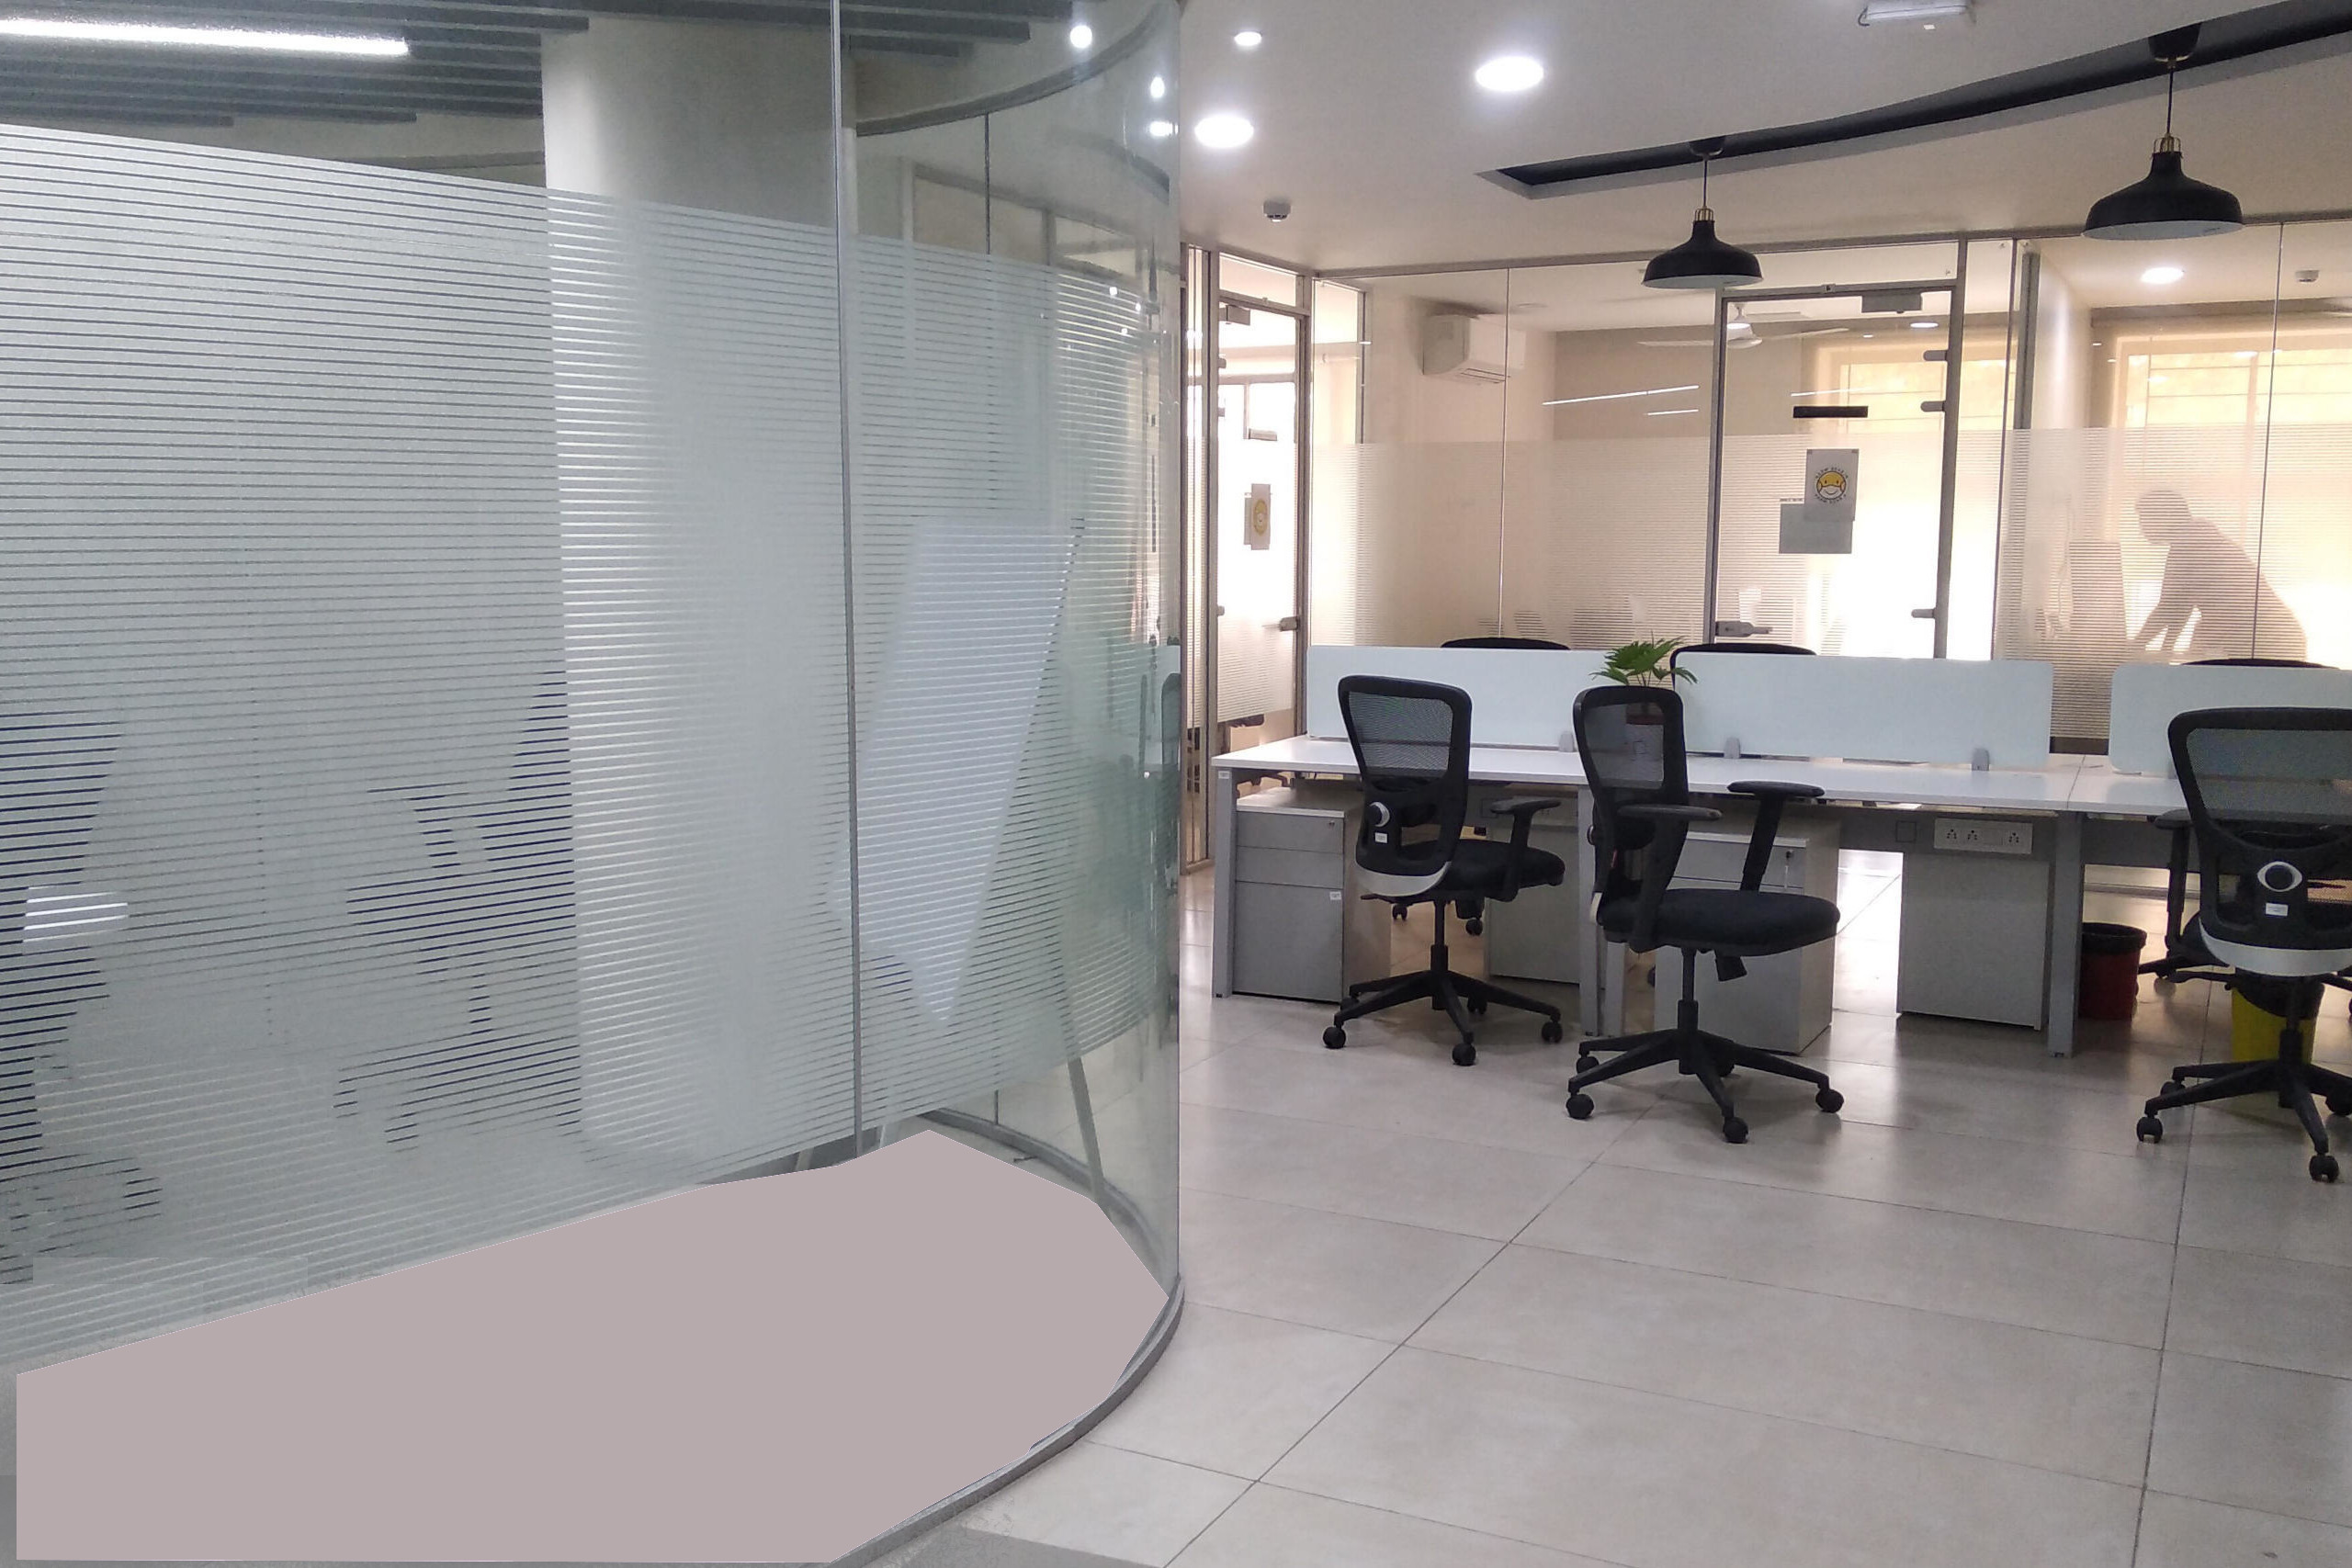
\includegraphics[height=\paperheight]{usach.jpg}}

\usetheme[sectionstyle=style3]{trigon}

% Definir los logotipos a utilizar (comentar si no hay logotipo)
\biglogo{usach_logo.jpg} % Se utiliza sólo en la portada
\smalllogo{_logo_small.png} % Se utiliza en la esquina superior derecha de los marcos normales

% ------ Si quieres cambiar los colores por defecto del tema, hazlo aquí ------
\definecolor{tPrim}{HTML}{eA0600}   % 716
\definecolor{tSec}{HTML}{3141B1}    % cool gray
\definecolor{tAccent}{HTML}{502F6C} % 294

 
% ------ Paquetes y definiciones utilizados para esta demostración. Se pueden eliminar ------
\usepackage{appendixnumberbeamer} % To use \appendix command
\pdfstringdefDisableCommands{% Fix hyperref translate warning with \appendix
\def\translate#1{#1}%
}
\usepackage{pgf-pie} % For pie charts 
\usepackage{caption} % For subfigures
\usepackage{subcaption} % For subfigures
\usepackage{xspace}
\newcommand{\themename}{\textbf{\textsc{USACHtheme}}\xspace}
\usepackage[scale=2]{ccicons} % Icons for CC-BY-SA
\usepackage{booktabs} % Better tables


%==============================================================================
%                               COMENZAR DOCUMENTO
%==============================================================================
\begin{document}

%--------------------------------------
% Create title frame
\titleframe

%--------------------------------------
% Table of contents
\begin{frame}{Overview}
  \setbeamertemplate{section in toc}[sections numbered]
  \tableofcontents[hideallsubsections]
\end{frame}



%==============================================
\section{SRISHTI - Summer Research Internship}
%==============================================

\subsection{Overview}
\begin{frame}[fragile=singleslide]{\insertsectionhead}
  \framesubtitle{\insertsubsectionhead}
\begin{center}
\begin{itemize}
\item Summer Internship Program at IIIT Hyderabad
\item Proposal of  Prof CV Jawahar, Dean (Research) - funded by DST
\item \textbf{Period : } 16 May to 30 June 2022
\item Over 8000+ applicants from all over India
\item 126 students absorbed into various research teams/projects/groups
\end{itemize}
\end{center}
\end{frame}


\subsection{Goals and Objectives}
\begin{frame}[fragile=singleslide]{\insertsectionhead}
  \framesubtitle{\insertsubsectionhead}
\begin{center}
\begin{itemize}
\item Goal : To imbibe spirit of inquiry and research in students
\item Objectives
\begin{itemize}
\item Help interns realise and improve cognitive, general and personal skills
\item Introduce interns to academic and research ambience of IIITH
\item Lay foundation for potential collaboration in future
\end{itemize}
\end{itemize}
\end{center}
\end{frame}



\subsection{Assistance}

\begin{frame}[fragile=singleslide]{\insertsectionhead - \insertsubsectionhead}
 \framesubtitle{\insertsubsectionhead}
\begin{center}
\begin{itemize}
\item Assistance to be rendered to all interns
\begin{itemize}
\item Availability of mentor for discussions
\item Access to resources, as like any other student
\item Place to sit and work
\item Food and accommodation (via iHub)
\item Invitation to special lectures, if any
\end{itemize}
\end{itemize}
\end{center}
\end{frame}

\subsection{SRISHTI 22}

\begin{frame}[fragile=singleslide]{\insertsectionhead - \insertsubsectionhead}
 % \framesubtitle{\insertsubsectionhead}
\begin{center}
\begin{itemize}
\item Monday,	16 May	:	Inauguration	(morning)			
\item Saturday,	21 May	:	Camp Fire	(evening)			
\item Saturday,	28 May	:	Invited Lecture	(evening)			
\item Saturday,	04 June	:	Talk to Research Heads (Panel)	(evening)				
\item Saturday,	11 June	:	Film Show and Review	(evening)			
\item Saturday,	18 June	:	Golconda Outing	(full day)			
\item Saturday,	25 June	:	Interns’ Evening	(evening)		
\item Thursday,	30 June	:	Valediction	(morning)	
\item Progress Monitoring on Wednesdays - 18 May, 25  May, 01 June, 08 June, 15 June, 22 June	 
\end{itemize}
\end{center}
\end{frame}




%-------------------------------------
%\end{document}
%--------------------------------------


\end{document}
